\documentclass[tikz]{standalone}

\usepackage{pgfplots}
\pgfplotsset{compat=1.15}
\usepackage{mathrsfs}
\usetikzlibrary{arrows,calc}
\usepackage{tkz-euclide}
\pagestyle{empty}

\definecolor{AngleClr}{rgb}{0,0.39215686274509803,0}
\definecolor{ShapeClr}{rgb}{0.6,0.2,0}

\begin{document}

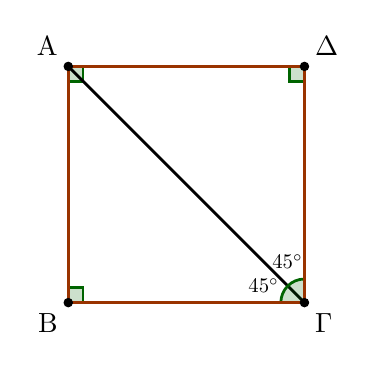
\begin{tikzpicture}[scale=.75]
\tkzSetUpLine[line width=1pt,color=black]
\tkzSetUpPoint[fill=black]

\tkzDefPoints{0/0/B,4/0/C,0/4/A,4/4/D,2/1.5/O}

\tkzFillPolygon[fill=white](A,B,C,D)

\tkzMarkRightAngles[line width=1pt, size=.25,color=AngleClr,fill=AngleClr,fill opacity=0.2](A,B,C C,D,A D,A,B)

\tkzDrawSegment(A,C)

\tkzFillAngles[fill=AngleClr,size=.4,fill opacity=0.2](D,C,A A,C,B)
\tkzMarkAngles[line width=1pt,size=.4,color=AngleClr](D,C,A A,C,B)
\tkzLabelAngles[scale=0.75](D,C,A A,C,B){$45^\circ$}

\tkzDrawPolygon[color=ShapeClr](A,B,C,D)
\tkzDrawPoints[size=3](A,B,C,D)
\tkzLabelPoint[above left](A){$\rm A$}
\tkzLabelPoint[below left](B){$\rm B$}
\tkzLabelPoint[below right](C){$\rm \Gamma$};
\tkzLabelPoint[above right](D){$\rm \Delta$};

\end{tikzpicture}
\end{document}
